\documentclass{article}
\usepackage{hyperref}
\usepackage{graphicx}
\usepackage{algorithm2e}

\begin{document}

\title{Raising \emph{Anopheles} hybrids}

\author{Erik Garrison}

\maketitle

\begin{abstract}
In this rotation I attempted to hybridize various species in the \emph{Anopheles gambiae} species complex, with the objective of eventually applying RNA sequencing to hybrid offspring to determine if particular features of gene regulation might be result from hybrid incompatibility.
\end{abstract}


\section{Hybrid incompatibility}

An understanding of the genetics of malarial vector species of \emph{Anopheles} is an important component of malarial eradication programs \cite{pmid25554792}. The major African vector, \emph{Anopheles gambiae} is a species complex formed of two main subspecies (labeled M and S) that appear to exist in near-total reproductive isolation  \cite{lanzaro2013speciation}.
This reproductive isolation has led to the suggestion that the complex may present an example of ongoing speciation, and recently the M and S forms have been reclassified as separate species, \emph{An. gambiae s.s.} (S form) and \emph{An. coluzzii} (M form) \cite{pmid26131476}.
These forms, as well as other \emph{Anopheles} species, can hybridize, but following Haldane's rule, males (which are the heterogametic sex) are sterile. In the case of \emph{An. gambiae s.s.} and \emph{An. arabiensis} QTL mapping suggests that this effect results from incompatibilites between loci on the X chromosome and the autosomes \cite{slotman2004genetics}.
In the interest of better-understanding the genomics of this incompatibility, we attempted to cross various laboratory-adapted \emph{Anopheles} strains. Several crosses eventually yielded adult mosquitoes, and I have retained these for possible RNA sequencing and analysis.

\section{Methods}

Five laboratory strains of mosquitoes were raised from eggs purchased from a supplier. Two experiments were undertaken. In the first, crosses were attempted between the following three strains:

\begin{itemize}
\item \emph{An. arabiensis} ``KGB'' (subsaharan Africa)
\item \emph{An. merus} ``merus'' (brackish, coastal)
\item \emph{An. quadrimaculatus} ``quad'' (North American)
\end{itemize}

In the second, we used only species of the \emph{gambiae} complex which have been shown to produce hybrid F1 offspring:

\begin{itemize}
\item \emph{An. coluzzii} ``Mali-NIH'' (formerly M form)
\item \emph{An. gambiae s.s.} Pimperena ``pimp'' (formely S form).
\end{itemize}

In both experiments, eggs were floated in net-covered trays filled with several centimeters of simulated pondwater. Larvae were fed with two kinds of fish food (liquifry and pellet) and monitored for developmental progress. Adults were collected immediately after hatching from the final larval stage. Speedy collection ensures that mating between pairs of the same species does not occur. Males are not capable of mating for several hours after hatching as the clasping aparatus that is essential for grasping the female genitalia is not functional.

Once collected, males and females were sorted by sex (which can be done easily with the aid of a dissecting microscope due to the distinct morphology of the sexes) and males and females of different species were placed in cages with glucose food. After several days, females were fed using donor blood placed in a petri dish covered in parafilm and heated to near human body temperature using warm water, however ``pimp'' females required live feeding on human donors. After another 24 to 48 hours, dishes with the same water used to raise larvae were placed in the cages to receive eggs. When a first feeding produced no eggs, a second round of feeding was attempted. (In one case anestitized mice were used, but no females fed by this method laid viable eggs.)

\section{Results}


\bibliography{references}{}

\bibliographystyle{plain}

\begin{figure}[p]

\begin{caption}
mali-NIH male / pimp female F1s
\end{caption}
\centering
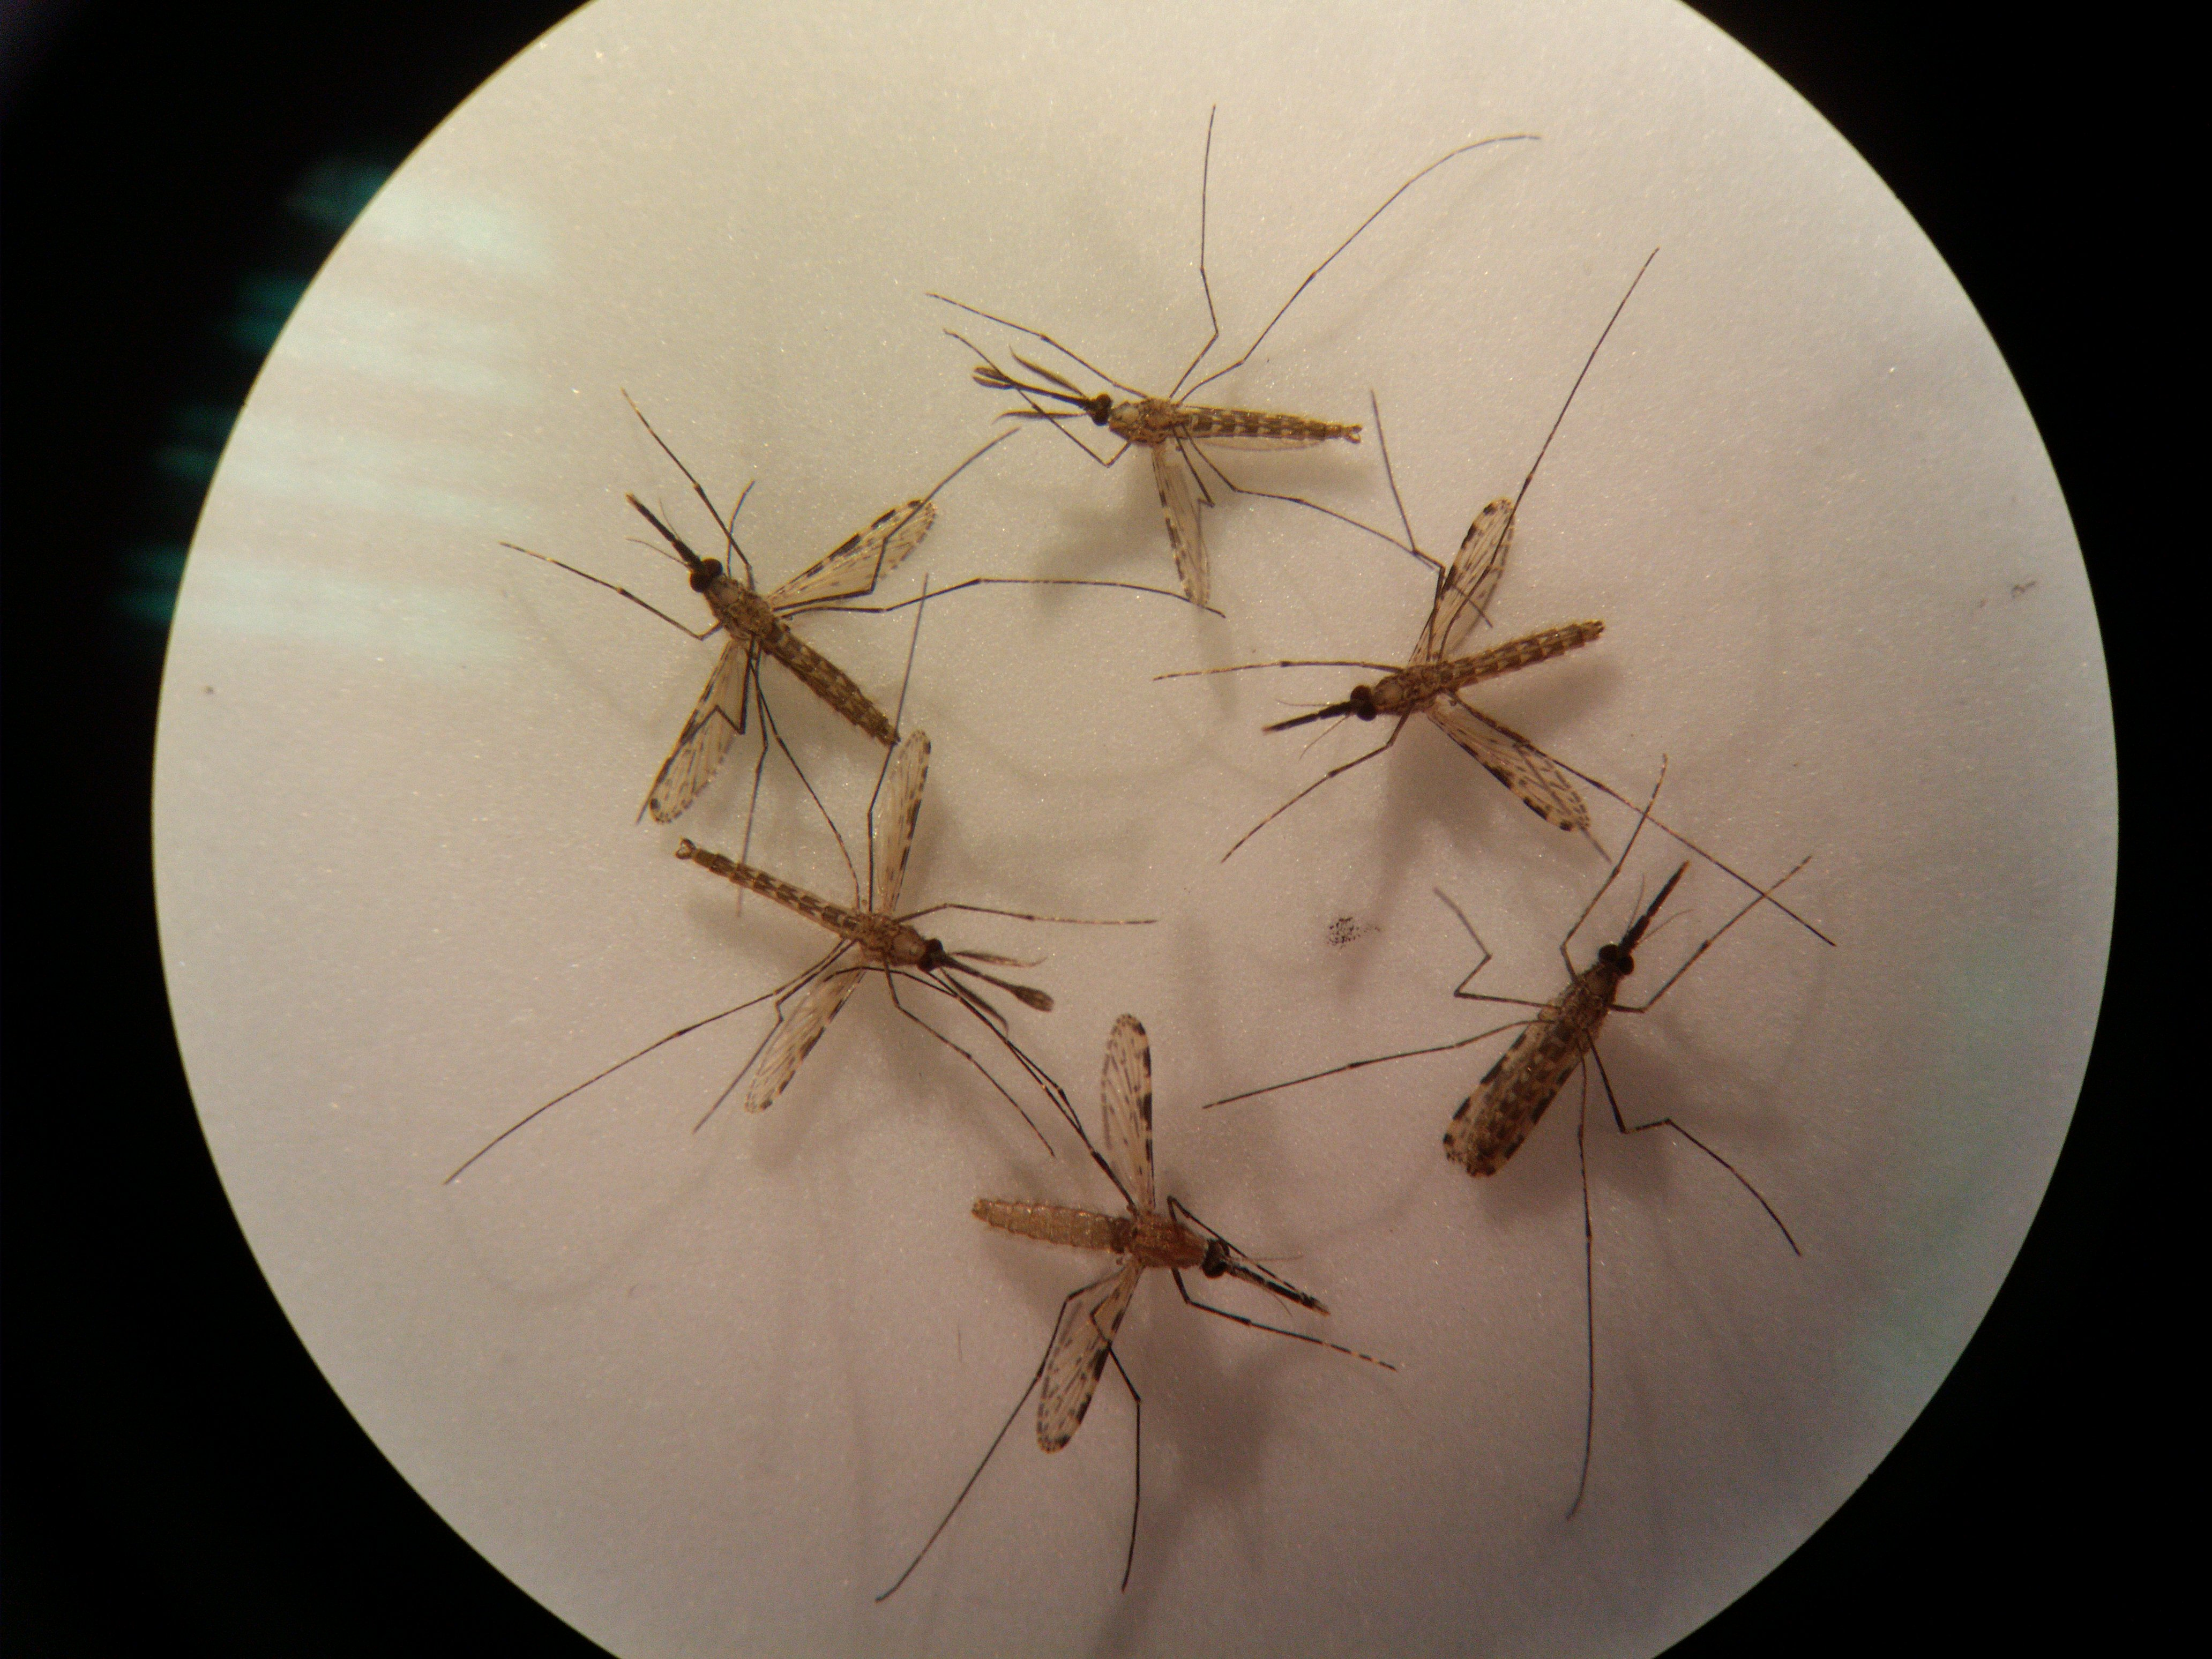
\includegraphics[scale=0.1]{mali-NIH-♂_pimp-♀}
\end{figure}

\begin{figure}[p]
\begin{caption}
pimp male / mali-nih female F1s
\end{caption}

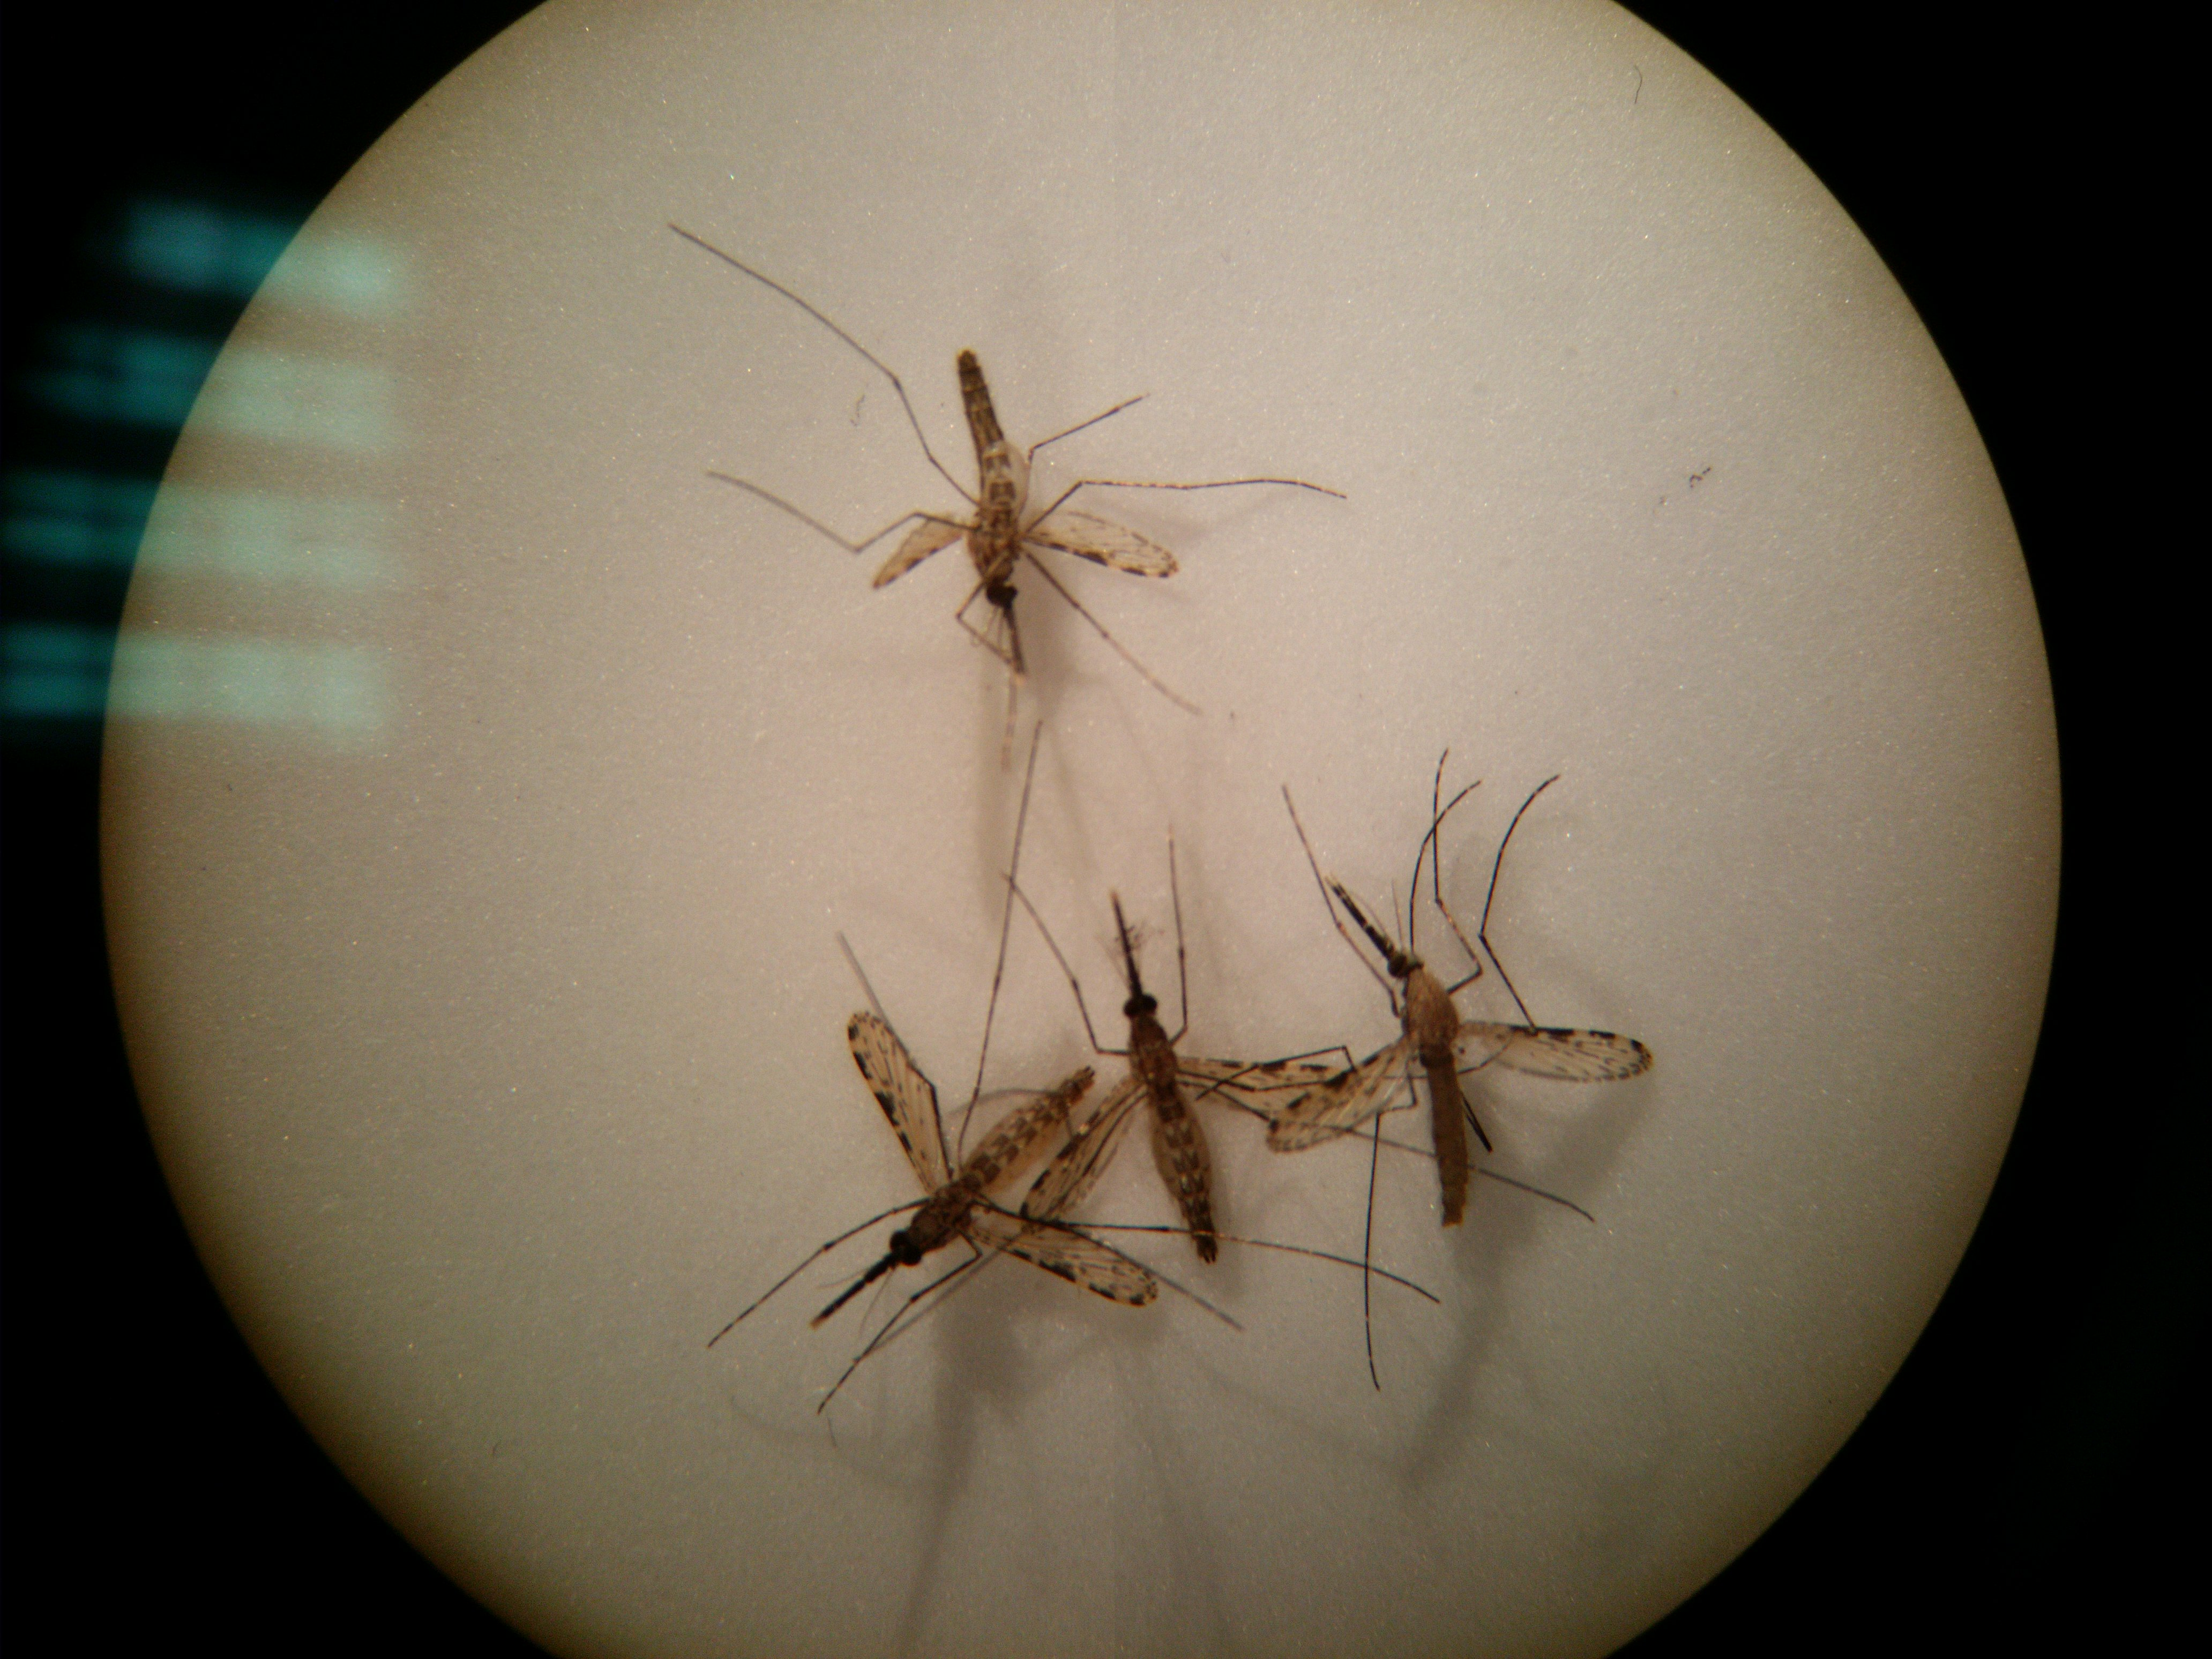
\includegraphics[scale=0.1]{pimp-♂_mali-NIH-♀}
\end{figure}

\end{document}
